\documentclass[12pt, a4paper]{article}
\usepackage[swedish]{babel}
\usepackage[version=4]{mhchem}
\usepackage{amsmath}
\usepackage[swedish]{varioref}
\usepackage{hyperref}
\hypersetup{
    colorlinks=true,
    linkcolor=black,
    pdftitle={Fysik 1 Uppslagverk},
    pdfpagemode=FullScreen
}
\usepackage[swedish]{cleveref}
\usepackage{amsthm}
\renewcommand\qedsymbol{V.S.V.}
\theoremstyle{definition}
\newtheorem{exm}{Exempel}
\usepackage{cancel}
\usepackage{float}
\usepackage{array}
\usepackage{enumitem}
\renewcommand{\labelitemii}{$\circ$}
\usepackage[margin=2.5cm]{geometry}
\usepackage{pgf}
\usepackage{tikz}
\usepackage{graphicx}
\usetikzlibrary{calc,decorations.pathmorphing,decorations.pathreplacing,calligraphy}
\usepackage{tcolorbox}
\tcbuselibrary{theorems}
\usepackage{array}

% Make the heart character work
\DeclareSymbolFont{extraup}{U}{zavm}{m}{n}
\DeclareMathSymbol{\varheartsuit}{\mathalpha}{extraup}{86}


\title{Sammanfattning - Fysik 1 \\ Blackebergs Gymnasium}
\author{Marcell Ziegler - NA21D}

\newcommand{\noref}{\textcolor{red}{\textbf{\textit{\underline{missing reference}}}}}

\begin{document}
    \begin{titlepage}
        \maketitle
        \centering
        \vfill
        
\includegraphics[width=0.6\textwidth]{title.jpg}
        \vfill
        \textbf{OBS!} Alla siffror/referenser som verkar vara länkar är antagligen länkar. Svåra/ogenomgångna matte-symboler borde också vara länkar som leder till förklaring, dock endast for första uppkomsten per ekvation. Tryck gärna om du undrar nåt!
    \end{titlepage}

    \tableofcontents

    \newpage

    \section*{Förord}
    Innan början finns det några viktiga saker att utreda för denna sammanfattning. Först av allt är detta ett fritidsprojekt och inte skolmaterial, därför finns det ingen garanti på att allt är 100\% rätt dock borde dokumentet överlag inte innehålla några större faktafel. Nästa punkt är att denna sammanfattning är gjord för effektivitet så alla förklaringar är inte fullständiga och huvuddelen innehåller inte fullständiga härledning och heller inte många räkneexempel. Om du söker fullständiga förklaring på vissa saker får du gärna titta i bilagorna mot slutet av dokumentet. Där hittar du även förklaringar till matematiska täcken som jag använder men som vi inte har gått igenom. Jag kommer heller inte förklara vanliga symboler för storheter som ex. massma ($m$) och hastighet ($v$).
    \begin{center}
        \large{Ha kul främst av allt, men kom ihåg likt vad Tor brukar säga:}\\
        \Large{Jag \textcolor{red}{$\varheartsuit$} Fysik!}
    \end{center}

    \part{Rörelse}
    \input{chapters/rörelse.tex}

    \part{Krafter}
    En kraft är en vektorstorhet, dvs. att den har en riktning, som oftast definieras som produkten av accelerationen och massan. Denna beskrivs av Newtons andra lag (N II)---\emph{kraftlagen}---som
    \begin{equation*}
        F=ma
    \end{equation*}
    Lägg märke till att vi inte använder vanlig vektornotation ($\vec{F}$) eftersom storleken av kraften är det man oftast söker, speciellt i denna kurs. Med detta menas att $F = |\vec{F}|$. Enheten för kraft är Newton (N) och beskrivs i grundenheter som $\frac{kg \cdot m}{s^2}$. När man söker riktningen av en kraft beskrivs detta nästan aldrig som en vektor ändå så denna fakta är mest för rätthet än nyttig användning.

    Det viktigaste som du kan veta om krafter är att enligt newtons lagar finns det alltid två av varje kraft. Han sade att ''varje kraft har en lika och motsatt \emph{reaktionskraft}'' (N III). Detta är exakt vad man tror det är. En kraft som verkar på ett föremål kommer att ha en reaktion från det föremålet i motsatt riktning med samma magnitud.

    Krafter kommer i många olika slag och de flesta från kursen finns förklarade nedan men en av de viktigaste och mest universella krafttyperna är normalkraften $N$ (mer sällsynt $F_n$). Denna är en kraft som är vinkelrät mot någon yta, dvs. normal mot ytan. Det finns enligt newtons tredje lag naturligtvis alltid två normalkrafter.
    \begin{exm}
        En låda sitter på ett bord under jordens gravitation (I verkligheten är alla krafter i en och samma vertikala linje men är separerade för visualiseringens skull). Alla krafter på bilden är lika stora och alla krafter har en lika och motsatt reaktionskraft. $F_g = -N$ då denna kraft är densamma som lådan verkar på bordet med och $N$ är lika stor men motsatt som rekation. Båda normalkrafter angriper vid kontaktytan medan $F_g$ angringer vid masscentrum.
        \begin{center}
            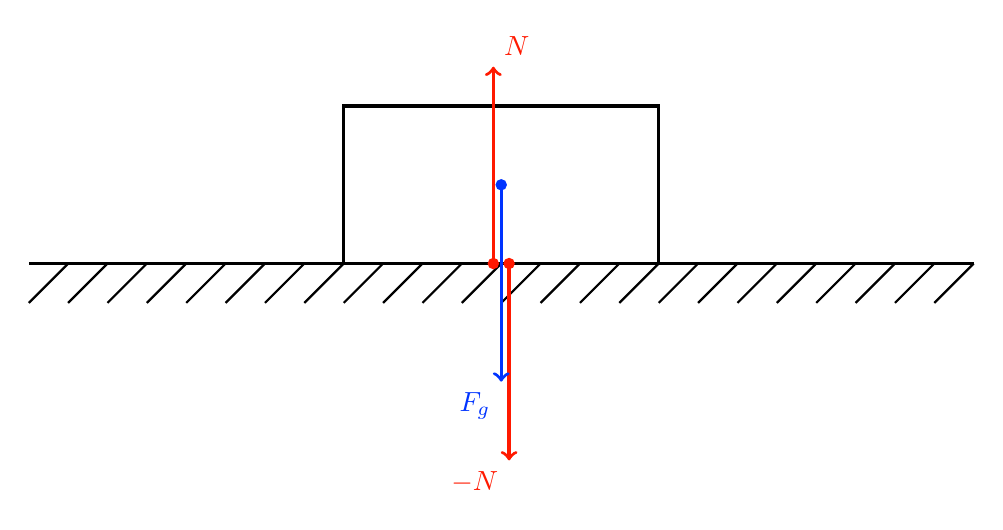
\begin{tikzpicture}
                \draw[thick] (-6,0) -- (6,0);
                \foreach \x in {-5.5,-5,...,6}  
                    \draw[thick] (\x,0) -- ++(-0.5,-0.5);
                \draw[very thick] (-2,2) rectangle (2,0);
                \draw[->, very thick, color=red!80!orange] (-0.1,0) -- ++(0,2.5) node [anchor=south west] {$N$};
                \filldraw[very thick, color=red!80!orange] (-0.1,0) circle [radius=0.05];
                \draw[->, very thick, color=red!80!orange] (0.1,0) -- ++(0,-2.5) node [anchor=north east] {$-N$};
                \filldraw[very thick, color=red!80!orange] (0.1,0) circle [radius=0.05];
                \draw[->, very thick, color=blue!80!cyan] (0,1) -- ++(0,-2.5) node [anchor=north east] {$F_g$};
                \filldraw[very thick, color=blue!80!cyan] (0,1) circle [radius=0.05];
            \end{tikzpicture}
        \end{center}
    \end{exm}

    \section{Tyngdkraften}
Tyngdkraften, bättre känd som gravitationen, är den kraft som två massor utgör på varandra enligt fysikens lagar. Den betecknas $F_g$ och har samma enhet som alla andra krafter. Formeln för tyngdkraften är följande:
\begin{equation*}
    F_g = G \cdot \frac{m_1m_2}{r^2}
\end{equation*}
$G$ är \emph{gravitationskonstanten} och har ett värde på $G \approx 6.67 \cdot 10^{-11}$, $m_1$ och $m_2$ är massorna av de två interagerande föremålen och $r$ är avstånden mellan deras masscentrum. Detta samband innebär att $F_g \hyperref[def:propto]{\propto} \frac{1}{r^2}$. Detta gör att tyngdkraft avtar myhcket snabbt när avståndet ökar.

\section{Friktionskraft}
Friktionskraften är den kraft som två föremål utgör på varandra när de är i kontakt och en yttre kraft verkar på ena föremålet medan en lika stor kraft inte verkar på det andra. Denna har beteckningen $F_f$ och har formeln
\begin{equation*}
    F_f = \mu N
\end{equation*}

    \newpage
    \appendix
    \section{Härledningar}
    \label{appendix:härledning}
    \input{chapters/härledningar.tex}
    \section{Exempel}
    \label{appendix:exempel}
\end{document}